% Created by tikzDevice version 0.10.1 on 2019-04-10 17:43:13
% !TEX encoding = UTF-8 Unicode
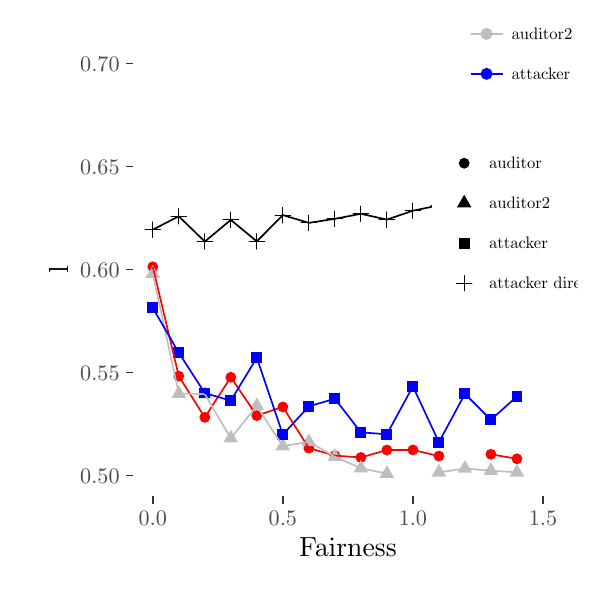
\begin{tikzpicture}[x=1pt,y=1pt]
\definecolor{fillColor}{RGB}{255,255,255}
\path[use as bounding box,fill=fillColor,fill opacity=0.00] (0,0) rectangle (198.74,198.74);
\begin{scope}
\path[clip] (  0.00,  0.00) rectangle (198.74,198.74);
\definecolor{drawColor}{RGB}{255,255,255}
\definecolor{fillColor}{RGB}{255,255,255}

\path[draw=drawColor,line width= 0.6pt,line join=round,line cap=round,fill=fillColor] ( -0.00,  0.00) rectangle (198.74,198.74);
\end{scope}
\begin{scope}
\path[clip] ( 38.16, 29.45) rectangle (193.24,193.24);
\definecolor{fillColor}{RGB}{255,0,0}

\path[fill=fillColor] ( 45.21,112.33) circle (  1.96);
\definecolor{fillColor}{RGB}{190,190,190}

\path[fill=fillColor] ( 45.21,112.92) --
	( 47.85,108.34) --
	( 42.56,108.34) --
	cycle;
\definecolor{fillColor}{RGB}{0,0,255}

\path[fill=fillColor] ( 43.24, 95.53) --
	( 47.17, 95.53) --
	( 47.17, 99.45) --
	( 43.24, 99.45) --
	cycle;
\definecolor{drawColor}{RGB}{0,0,0}

\path[draw=drawColor,line width= 0.4pt,line join=round,line cap=round] ( 42.43,125.74) -- ( 47.98,125.74);

\path[draw=drawColor,line width= 0.4pt,line join=round,line cap=round] ( 45.21,122.97) -- ( 45.21,128.52);
\definecolor{fillColor}{RGB}{255,0,0}

\path[fill=fillColor] ( 54.60, 72.83) circle (  1.96);
\definecolor{fillColor}{RGB}{190,190,190}

\path[fill=fillColor] ( 54.60, 69.53) --
	( 57.25, 64.96) --
	( 51.96, 64.96) --
	cycle;
\definecolor{fillColor}{RGB}{0,0,255}

\path[fill=fillColor] ( 52.64, 79.34) --
	( 56.57, 79.34) --
	( 56.57, 83.27) --
	( 52.64, 83.27) --
	cycle;

\path[draw=drawColor,line width= 0.4pt,line join=round,line cap=round] ( 51.83,130.58) -- ( 57.38,130.58);

\path[draw=drawColor,line width= 0.4pt,line join=round,line cap=round] ( 54.60,127.81) -- ( 54.60,133.36);
\definecolor{fillColor}{RGB}{255,0,0}

\path[fill=fillColor] ( 64.00, 57.93) circle (  1.96);
\definecolor{fillColor}{RGB}{190,190,190}

\path[fill=fillColor] ( 64.00, 69.40) --
	( 66.65, 64.83) --
	( 61.36, 64.83) --
	cycle;
\definecolor{fillColor}{RGB}{0,0,255}

\path[fill=fillColor] ( 62.04, 64.75) --
	( 65.97, 64.75) --
	( 65.97, 68.68) --
	( 62.04, 68.68) --
	cycle;

\path[draw=drawColor,line width= 0.4pt,line join=round,line cap=round] ( 61.23,121.46) -- ( 66.78,121.46);

\path[draw=drawColor,line width= 0.4pt,line join=round,line cap=round] ( 64.00,118.69) -- ( 64.00,124.24);
\definecolor{fillColor}{RGB}{255,0,0}

\path[fill=fillColor] ( 73.40, 72.42) circle (  1.96);
\definecolor{fillColor}{RGB}{190,190,190}

\path[fill=fillColor] ( 73.40, 53.43) --
	( 76.05, 48.86) --
	( 70.76, 48.86) --
	cycle;
\definecolor{fillColor}{RGB}{0,0,255}

\path[fill=fillColor] ( 71.44, 61.99) --
	( 75.37, 61.99) --
	( 75.37, 65.92) --
	( 71.44, 65.92) --
	cycle;

\path[draw=drawColor,line width= 0.4pt,line join=round,line cap=round] ( 70.63,129.27) -- ( 76.18,129.27);

\path[draw=drawColor,line width= 0.4pt,line join=round,line cap=round] ( 73.40,126.50) -- ( 73.40,132.05);
\definecolor{fillColor}{RGB}{255,0,0}

\path[fill=fillColor] ( 82.80, 58.56) circle (  1.96);
\definecolor{fillColor}{RGB}{190,190,190}

\path[fill=fillColor] ( 82.80, 65.11) --
	( 85.44, 60.53) --
	( 80.16, 60.53) --
	cycle;
\definecolor{fillColor}{RGB}{0,0,255}

\path[fill=fillColor] ( 80.84, 77.51) --
	( 84.76, 77.51) --
	( 84.76, 81.43) --
	( 80.84, 81.43) --
	cycle;

\path[draw=drawColor,line width= 0.4pt,line join=round,line cap=round] ( 80.03,121.52) -- ( 85.58,121.52);

\path[draw=drawColor,line width= 0.4pt,line join=round,line cap=round] ( 82.80,118.75) -- ( 82.80,124.30);
\definecolor{fillColor}{RGB}{255,0,0}

\path[fill=fillColor] ( 92.20, 61.70) circle (  1.96);
\definecolor{fillColor}{RGB}{190,190,190}

\path[fill=fillColor] ( 92.20, 50.56) --
	( 94.84, 45.99) --
	( 89.56, 45.99) --
	cycle;
\definecolor{fillColor}{RGB}{0,0,255}

\path[fill=fillColor] ( 90.24, 49.75) --
	( 94.16, 49.75) --
	( 94.16, 53.67) --
	( 90.24, 53.67) --
	cycle;

\path[draw=drawColor,line width= 0.4pt,line join=round,line cap=round] ( 89.43,131.02) -- ( 94.98,131.02);

\path[draw=drawColor,line width= 0.4pt,line join=round,line cap=round] ( 92.20,128.24) -- ( 92.20,133.79);
\definecolor{fillColor}{RGB}{255,0,0}

\path[fill=fillColor] (101.60, 46.82) circle (  1.96);
\definecolor{fillColor}{RGB}{190,190,190}

\path[fill=fillColor] (101.60, 52.14) --
	(104.24, 47.56) --
	( 98.96, 47.56) --
	cycle;
\definecolor{fillColor}{RGB}{0,0,255}

\path[fill=fillColor] ( 99.64, 59.95) --
	(103.56, 59.95) --
	(103.56, 63.87) --
	( 99.64, 63.87) --
	cycle;

\path[draw=drawColor,line width= 0.4pt,line join=round,line cap=round] ( 98.83,128.20) -- (104.38,128.20);

\path[draw=drawColor,line width= 0.4pt,line join=round,line cap=round] (101.60,125.42) -- (101.60,130.97);
\definecolor{fillColor}{RGB}{255,0,0}

\path[fill=fillColor] (111.00, 44.11) circle (  1.96);
\definecolor{fillColor}{RGB}{190,190,190}

\path[fill=fillColor] (111.00, 46.76) --
	(113.64, 42.18) --
	(108.36, 42.18) --
	cycle;
\definecolor{fillColor}{RGB}{0,0,255}

\path[fill=fillColor] (109.04, 62.70) --
	(112.96, 62.70) --
	(112.96, 66.63) --
	(109.04, 66.63) --
	cycle;

\path[draw=drawColor,line width= 0.4pt,line join=round,line cap=round] (108.22,129.66) -- (113.77,129.66);

\path[draw=drawColor,line width= 0.4pt,line join=round,line cap=round] (111.00,126.88) -- (111.00,132.43);
\definecolor{fillColor}{RGB}{255,0,0}

\path[fill=fillColor] (120.40, 43.43) circle (  1.96);
\definecolor{fillColor}{RGB}{190,190,190}

\path[fill=fillColor] (120.40, 42.60) --
	(123.04, 38.03) --
	(117.76, 38.03) --
	cycle;
\definecolor{fillColor}{RGB}{0,0,255}

\path[fill=fillColor] (118.44, 50.55) --
	(122.36, 50.55) --
	(122.36, 54.48) --
	(118.44, 54.48) --
	cycle;

\path[draw=drawColor,line width= 0.4pt,line join=round,line cap=round] (117.62,131.48) -- (123.17,131.48);

\path[draw=drawColor,line width= 0.4pt,line join=round,line cap=round] (120.40,128.71) -- (120.40,134.26);
\definecolor{fillColor}{RGB}{255,0,0}

\path[fill=fillColor] (129.80, 46.12) circle (  1.96);
\definecolor{fillColor}{RGB}{190,190,190}

\path[fill=fillColor] (129.80, 40.65) --
	(132.44, 36.08) --
	(127.16, 36.08) --
	cycle;
\definecolor{fillColor}{RGB}{0,0,255}

\path[fill=fillColor] (127.84, 49.85) --
	(131.76, 49.85) --
	(131.76, 53.77) --
	(127.84, 53.77) --
	cycle;

\path[draw=drawColor,line width= 0.4pt,line join=round,line cap=round] (127.02,129.39) -- (132.57,129.39);

\path[draw=drawColor,line width= 0.4pt,line join=round,line cap=round] (129.80,126.62) -- (129.80,132.16);
\definecolor{fillColor}{RGB}{255,0,0}

\path[fill=fillColor] (139.20, 46.15) circle (  1.96);
\definecolor{fillColor}{RGB}{0,0,255}

\path[fill=fillColor] (137.24, 67.17) --
	(141.16, 67.17) --
	(141.16, 71.10) --
	(137.24, 71.10) --
	cycle;

\path[draw=drawColor,line width= 0.4pt,line join=round,line cap=round] (136.42,132.60) -- (141.97,132.60);

\path[draw=drawColor,line width= 0.4pt,line join=round,line cap=round] (139.20,129.82) -- (139.20,135.37);
\definecolor{fillColor}{RGB}{255,0,0}

\path[fill=fillColor] (148.60, 43.94) circle (  1.96);
\definecolor{fillColor}{RGB}{190,190,190}

\path[fill=fillColor] (148.60, 41.10) --
	(151.24, 36.52) --
	(145.95, 36.52) --
	cycle;
\definecolor{fillColor}{RGB}{0,0,255}

\path[fill=fillColor] (146.63, 46.95) --
	(150.56, 46.95) --
	(150.56, 50.88) --
	(146.63, 50.88) --
	cycle;

\path[draw=drawColor,line width= 0.4pt,line join=round,line cap=round] (145.82,134.54) -- (151.37,134.54);

\path[draw=drawColor,line width= 0.4pt,line join=round,line cap=round] (148.60,131.76) -- (148.60,137.31);
\definecolor{fillColor}{RGB}{190,190,190}

\path[fill=fillColor] (158.00, 42.50) --
	(160.64, 37.92) --
	(155.35, 37.92) --
	cycle;
\definecolor{fillColor}{RGB}{0,0,255}

\path[fill=fillColor] (156.03, 64.47) --
	(159.96, 64.47) --
	(159.96, 68.40) --
	(156.03, 68.40) --
	cycle;

\path[draw=drawColor,line width= 0.4pt,line join=round,line cap=round] (155.22,126.14) -- (160.77,126.14);

\path[draw=drawColor,line width= 0.4pt,line join=round,line cap=round] (158.00,123.37) -- (158.00,128.92);
\definecolor{fillColor}{RGB}{255,0,0}

\path[fill=fillColor] (167.39, 44.60) circle (  1.96);
\definecolor{fillColor}{RGB}{190,190,190}

\path[fill=fillColor] (167.39, 41.70) --
	(170.04, 37.12) --
	(164.75, 37.12) --
	cycle;
\definecolor{fillColor}{RGB}{0,0,255}

\path[fill=fillColor] (165.43, 55.09) --
	(169.36, 55.09) --
	(169.36, 59.01) --
	(165.43, 59.01) --
	cycle;

\path[draw=drawColor,line width= 0.4pt,line join=round,line cap=round] (164.62,130.72) -- (170.17,130.72);

\path[draw=drawColor,line width= 0.4pt,line join=round,line cap=round] (167.39,127.94) -- (167.39,133.49);
\definecolor{fillColor}{RGB}{255,0,0}

\path[fill=fillColor] (176.79, 42.95) circle (  1.96);
\definecolor{fillColor}{RGB}{190,190,190}

\path[fill=fillColor] (176.79, 41.11) --
	(179.44, 36.53) --
	(174.15, 36.53) --
	cycle;
\definecolor{fillColor}{RGB}{0,0,255}

\path[fill=fillColor] (174.83, 63.52) --
	(178.76, 63.52) --
	(178.76, 67.45) --
	(174.83, 67.45) --
	cycle;

\path[draw=drawColor,line width= 0.4pt,line join=round,line cap=round] (174.02,132.32) -- (179.57,132.32);

\path[draw=drawColor,line width= 0.4pt,line join=round,line cap=round] (176.79,129.54) -- (176.79,135.09);
\definecolor{drawColor}{RGB}{255,0,0}

\path[draw=drawColor,line width= 0.6pt,line join=round] ( 45.21,112.33) --
	( 54.60, 72.83) --
	( 64.00, 57.93) --
	( 73.40, 72.42) --
	( 82.80, 58.56) --
	( 92.20, 61.70) --
	(101.60, 46.82) --
	(111.00, 44.11) --
	(120.40, 43.43) --
	(129.80, 46.12) --
	(139.20, 46.15) --
	(148.60, 43.94);

\path[draw=drawColor,line width= 0.6pt,line join=round] (167.39, 44.60) --
	(176.79, 42.95);
\definecolor{drawColor}{RGB}{190,190,190}

\path[draw=drawColor,line width= 0.6pt,line join=round] ( 45.21,109.87) --
	( 54.60, 66.48) --
	( 64.00, 66.35) --
	( 73.40, 50.38) --
	( 82.80, 62.06) --
	( 92.20, 47.51) --
	(101.60, 49.09) --
	(111.00, 43.71) --
	(120.40, 39.55) --
	(129.80, 37.60);

\path[draw=drawColor,line width= 0.6pt,line join=round] (148.60, 38.05) --
	(158.00, 39.45) --
	(167.39, 38.65) --
	(176.79, 38.05);
\definecolor{drawColor}{RGB}{0,0,255}

\path[draw=drawColor,line width= 0.6pt,line join=round] ( 45.21, 97.49) --
	( 54.60, 81.30) --
	( 64.00, 66.71) --
	( 73.40, 63.96) --
	( 82.80, 79.47) --
	( 92.20, 51.71) --
	(101.60, 61.91) --
	(111.00, 64.67) --
	(120.40, 52.52) --
	(129.80, 51.81) --
	(139.20, 69.13) --
	(148.60, 48.92) --
	(158.00, 66.43) --
	(167.39, 57.05) --
	(176.79, 65.49);
\definecolor{drawColor}{RGB}{0,0,0}

\path[draw=drawColor,line width= 0.6pt,line join=round] ( 45.21,125.74) --
	( 54.60,130.58) --
	( 64.00,121.46) --
	( 73.40,129.27) --
	( 82.80,121.52) --
	( 92.20,131.02) --
	(101.60,128.20) --
	(111.00,129.66) --
	(120.40,131.48) --
	(129.80,129.39) --
	(139.20,132.60) --
	(148.60,134.54) --
	(158.00,126.14) --
	(167.39,130.72) --
	(176.79,132.32);
\end{scope}
\begin{scope}
\path[clip] (  0.00,  0.00) rectangle (198.74,198.74);
\definecolor{drawColor}{gray}{0.30}

\node[text=drawColor,anchor=base east,inner sep=0pt, outer sep=0pt, scale=  0.80] at ( 33.21, 34.14) {0.50};

\node[text=drawColor,anchor=base east,inner sep=0pt, outer sep=0pt, scale=  0.80] at ( 33.21, 71.36) {0.55};

\node[text=drawColor,anchor=base east,inner sep=0pt, outer sep=0pt, scale=  0.80] at ( 33.21,108.59) {0.60};

\node[text=drawColor,anchor=base east,inner sep=0pt, outer sep=0pt, scale=  0.80] at ( 33.21,145.82) {0.65};

\node[text=drawColor,anchor=base east,inner sep=0pt, outer sep=0pt, scale=  0.80] at ( 33.21,183.04) {0.70};
\end{scope}
\begin{scope}
\path[clip] (  0.00,  0.00) rectangle (198.74,198.74);
\definecolor{drawColor}{gray}{0.20}

\path[draw=drawColor,line width= 0.6pt,line join=round] ( 35.41, 36.89) --
	( 38.16, 36.89);

\path[draw=drawColor,line width= 0.6pt,line join=round] ( 35.41, 74.12) --
	( 38.16, 74.12);

\path[draw=drawColor,line width= 0.6pt,line join=round] ( 35.41,111.34) --
	( 38.16,111.34);

\path[draw=drawColor,line width= 0.6pt,line join=round] ( 35.41,148.57) --
	( 38.16,148.57);

\path[draw=drawColor,line width= 0.6pt,line join=round] ( 35.41,185.80) --
	( 38.16,185.80);
\end{scope}
\begin{scope}
\path[clip] (  0.00,  0.00) rectangle (198.74,198.74);
\definecolor{drawColor}{gray}{0.20}

\path[draw=drawColor,line width= 0.6pt,line join=round] ( 45.21, 26.70) --
	( 45.21, 29.45);

\path[draw=drawColor,line width= 0.6pt,line join=round] ( 92.20, 26.70) --
	( 92.20, 29.45);

\path[draw=drawColor,line width= 0.6pt,line join=round] (139.20, 26.70) --
	(139.20, 29.45);

\path[draw=drawColor,line width= 0.6pt,line join=round] (186.19, 26.70) --
	(186.19, 29.45);
\end{scope}
\begin{scope}
\path[clip] (  0.00,  0.00) rectangle (198.74,198.74);
\definecolor{drawColor}{gray}{0.30}

\node[text=drawColor,anchor=base,inner sep=0pt, outer sep=0pt, scale=  0.80] at ( 45.21, 18.99) {0.0};

\node[text=drawColor,anchor=base,inner sep=0pt, outer sep=0pt, scale=  0.80] at ( 92.20, 18.99) {0.5};

\node[text=drawColor,anchor=base,inner sep=0pt, outer sep=0pt, scale=  0.80] at (139.20, 18.99) {1.0};

\node[text=drawColor,anchor=base,inner sep=0pt, outer sep=0pt, scale=  0.80] at (186.19, 18.99) {1.5};
\end{scope}
\begin{scope}
\path[clip] (  0.00,  0.00) rectangle (198.74,198.74);
\definecolor{drawColor}{RGB}{0,0,0}

\node[text=drawColor,anchor=base,inner sep=0pt, outer sep=0pt, scale=  1.00] at (115.70,  7.70) {Fairness};
\end{scope}
\begin{scope}
\path[clip] (  0.00,  0.00) rectangle (198.74,198.74);
\definecolor{drawColor}{RGB}{0,0,0}

\node[text=drawColor,rotate= 90.00,anchor=base,inner sep=0pt, outer sep=0pt, scale=  1.00] at ( 14.59,111.34) {l};
\end{scope}
\begin{scope}
\path[clip] (  0.00,  0.00) rectangle (198.74,198.74);
\definecolor{fillColor}{RGB}{255,255,255}

\path[fill=fillColor] (154.33,170.56) rectangle (201.14,226.07);
\end{scope}
\begin{scope}
\path[clip] (  0.00,  0.00) rectangle (198.74,198.74);
\definecolor{drawColor}{RGB}{190,190,190}
\definecolor{fillColor}{RGB}{190,190,190}

\path[draw=drawColor,line width= 0.4pt,line join=round,line cap=round,fill=fillColor] (165.82,196.50) circle (  1.96);
\end{scope}
\begin{scope}
\path[clip] (  0.00,  0.00) rectangle (198.74,198.74);
\definecolor{drawColor}{RGB}{190,190,190}

\path[draw=drawColor,line width= 0.6pt,line join=round] (160.04,196.50) -- (171.61,196.50);
\end{scope}
\begin{scope}
\path[clip] (  0.00,  0.00) rectangle (198.74,198.74);
\definecolor{drawColor}{RGB}{0,0,255}
\definecolor{fillColor}{RGB}{0,0,255}

\path[draw=drawColor,line width= 0.4pt,line join=round,line cap=round,fill=fillColor] (165.82,182.05) circle (  1.96);
\end{scope}
\begin{scope}
\path[clip] (  0.00,  0.00) rectangle (198.74,198.74);
\definecolor{drawColor}{RGB}{0,0,255}

\path[draw=drawColor,line width= 0.6pt,line join=round] (160.04,182.05) -- (171.61,182.05);
\end{scope}
\begin{scope}
\path[clip] (  0.00,  0.00) rectangle (198.74,198.74);
\definecolor{drawColor}{RGB}{0,0,0}

\node[text=drawColor,anchor=base west,inner sep=0pt, outer sep=0pt, scale=  0.60] at (174.86,194.44) {auditor2};
\end{scope}
\begin{scope}
\path[clip] (  0.00,  0.00) rectangle (198.74,198.74);
\definecolor{drawColor}{RGB}{0,0,0}

\node[text=drawColor,anchor=base west,inner sep=0pt, outer sep=0pt, scale=  0.60] at (174.86,179.98) {attacker};
\end{scope}
\begin{scope}
\path[clip] (  0.00,  0.00) rectangle (198.74,198.74);
\definecolor{fillColor}{RGB}{255,255,255}

\path[fill=fillColor] (146.24, 94.90) rectangle (209.23,164.87);
\end{scope}
\begin{scope}
\path[clip] (  0.00,  0.00) rectangle (198.74,198.74);
\definecolor{fillColor}{RGB}{0,0,0}

\path[fill=fillColor] (157.73,149.76) circle (  1.96);
\end{scope}
\begin{scope}
\path[clip] (  0.00,  0.00) rectangle (198.74,198.74);
\definecolor{fillColor}{RGB}{0,0,0}

\path[fill=fillColor] (157.73,138.35) --
	(160.38,133.78) --
	(155.09,133.78) --
	cycle;
\end{scope}
\begin{scope}
\path[clip] (  0.00,  0.00) rectangle (198.74,198.74);
\definecolor{fillColor}{RGB}{0,0,0}

\path[fill=fillColor] (155.77,118.89) --
	(159.70,118.89) --
	(159.70,122.81) --
	(155.77,122.81) --
	cycle;
\end{scope}
\begin{scope}
\path[clip] (  0.00,  0.00) rectangle (198.74,198.74);
\definecolor{drawColor}{RGB}{0,0,0}

\path[draw=drawColor,line width= 0.4pt,line join=round,line cap=round] (154.96,106.39) -- (160.51,106.39);

\path[draw=drawColor,line width= 0.4pt,line join=round,line cap=round] (157.73,103.62) -- (157.73,109.17);
\end{scope}
\begin{scope}
\path[clip] (  0.00,  0.00) rectangle (198.74,198.74);
\definecolor{drawColor}{RGB}{0,0,0}

\node[text=drawColor,anchor=base west,inner sep=0pt, outer sep=0pt, scale=  0.60] at (166.77,147.69) {auditor};
\end{scope}
\begin{scope}
\path[clip] (  0.00,  0.00) rectangle (198.74,198.74);
\definecolor{drawColor}{RGB}{0,0,0}

\node[text=drawColor,anchor=base west,inner sep=0pt, outer sep=0pt, scale=  0.60] at (166.77,133.24) {auditor2};
\end{scope}
\begin{scope}
\path[clip] (  0.00,  0.00) rectangle (198.74,198.74);
\definecolor{drawColor}{RGB}{0,0,0}

\node[text=drawColor,anchor=base west,inner sep=0pt, outer sep=0pt, scale=  0.60] at (166.77,118.78) {attacker};
\end{scope}
\begin{scope}
\path[clip] (  0.00,  0.00) rectangle (198.74,198.74);
\definecolor{drawColor}{RGB}{0,0,0}

\node[text=drawColor,anchor=base west,inner sep=0pt, outer sep=0pt, scale=  0.60] at (166.77,104.33) {attacker direct};
\end{scope}
\end{tikzpicture}
